%%
%% $Id$
%%
%% Copyright (c) 2007-2008 Christian Fehler
%% Copyright (c) 2007-2008 Benjamin Mies
%%


\chapter{Perspektive}\label{Perspective}

In diesem Kapitel werden die Zukunftsperspektiven für das \gtitool besprochen.
Bei der Implementierung wurde besonderer Wert darauf gelegt, dass das \gtitool
leicht zu erweitern sein muss. Der dadurch entstandene Aufwand konnte dadurch
gerechtfertigt werden, dass Erweiterungen in der Zukunft leichter und somit
schneller integriert werden können.\vspace{10pt}


\section{Graphische Komponenten}\label{PerspectiveGraphics}

Wie in Abschnitt \ref{Graph} beschrieben, verwenden wir zur graphischen
Darstellung der Automaten die Bibliothek JGraph. Diese Bibliothek bietet einen
sehr großen Funktionsumfang, der von uns nicht komplett ausgeschöpft werden
musste. Eine mögliche Implementierung für die Zukunft wäre es, diese Bibliothek
durch eine eigene Implementierung zu ersetzen, die dann nur den gewünschten
Umfang bietet und somit leichter zu warten und zu erweitern ist.\vspace{10pt}

Da eine solche Implementierung sehr viel Zeit in Anspruch nehmen würde, war es
uns im Rahmen der Diplomarbeit nicht möglich, neben den umgesetzten Komponenten
auch noch die graphischen Komponenten selbst zu implementieren. JGraph bot uns
die Möglichkeit sehr schnell und einfach bereits brauchbare Ergebnisse zu
erzielen. Es mussten einige in Abschnitt \ref{GraphJGraphAdaptation} beschriebene
Anpassungen vorgenommen werden, damit das Ergebnis unseren Vorstellungen
entsprach, diese waren aber im Gegensatz zu einer vollständigen Implementieren
zeitlich nicht so komplex.\vspace{10pt}

Zu einer möglichen Umsetzung ist zu sagen, dass sowohl Zustände wie auch
Übergänge implementiert werden müssen. Was gerade bei der Verwendung von
parallelen Übergängen ein größeres Problem sein könnte, da dort die Übergänge
nicht auf einer Linie verlaufen. Der größte Nutzer bei einer eigenständigen
Implementierung wäre, dass Änderungen leichter eingepflegt werden könnten, da
dies bei der sehr komplexen Implementierung von JGraph meistens problematisch
war.\vspace{10pt}

Ein weiterer Punkt betrifft die Übergänge. Im Moment verlaufen diese immer
gerade, außer bei parallelen Übergängen. Es wäre aber durchaus wünschenswert,
wenn die Übergänge zum Beispiel um einen Zustand herumgehen würden, wenn dieser
auf dem direkten Weg zwischen zwei Zuständen liegen würde.\vspace{10pt}


\section{Reguläre Ausdrücke}\label{PerspectiveRegEx}

Die wohl wichtigste und komplexeste Erweiterung, die für die Zukunft geplant
ist, ist die Unterstützung von regulären Ausdrücken. Der Benutzer soll somit in
der Lage sein, einen regulären Ausdruck wie
(\Symbol{a}$\mid$\Symbol{b})*\Symbol{a}\Symbol{b}\Symbol{b} eingeben zu können.
Anschließend sollen im Idealfall mehrere Möglichkeiten bestehen, mit diesem
Ausdruck weiter zu arbeiten. Diese Möglichkeiten sollen nun kurz angesprochen
werden.\vspace{10pt}

%### removes texlipse warning
Der eingegebene reguläre Ausdrucks soll mit dem in \cite[S.159ff]{Compilers}
beschriebenen McNaughton-Yamada-Thompson Algorithmus in einen Automaten
umgewandelt werden können. Diese Umwandlung sollte, wie die anderen Umwandlungen
auch, schrittweise durchgeführt werden. Dadurch soll es dem Benutzer ermöglicht
werden, den zur Umwandlung benutzten Algorithmus besser zu verstehen. Abbildung
\ref{FigureThompson} zeigt das Ergebnis, das bei einer solchen Umwandlung
entstehen würde.\vspace{10pt}
%### removes texlipse warning

\begin{figure}[h!]
\begin{center}
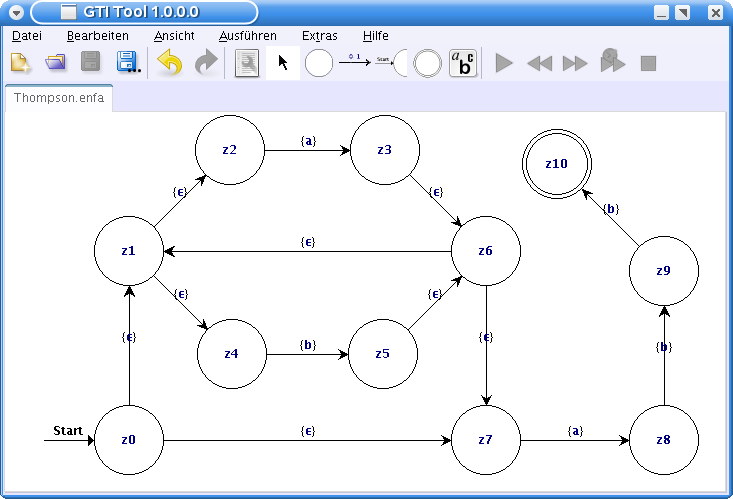
\includegraphics[width=12cm]{../images/thompson.png}
\caption{McNaughton-Yamada-Thompson Algorithmus}
\label{FigureThompson}
\end{center}
\end{figure}
\vspace{10pt}

%### removes texlipse warning
Eine weitere Verwendungsmöglichkeit eines regulären Ausdruck wäre das direkte
Umwandeln in einen DEA. Dieser Algorithmus wird in
\cite[S. 175ff]{Compilers} beschrieben und verwendet die Funktionen
\textit{nullable}, \textit{firstpos}, \textit{lastpos} und \textit{followpos},
um die Umwandlung durchzuführen. Bei der Umsetzung müsste das Berechnen dieser
Funktionen in irgendeiner Weise dargestellt werden, idealerweise anhand des
Syntaxbaumes des regulären Ausdrucks. Ein mögliches Ergebnis der direkten
Umwandlung ist in Abbildung \ref{FigureRegExDFA} zu sehen.\vspace{10pt}
%### removes texlipse warning

\begin{figure}[h!]
\begin{center}
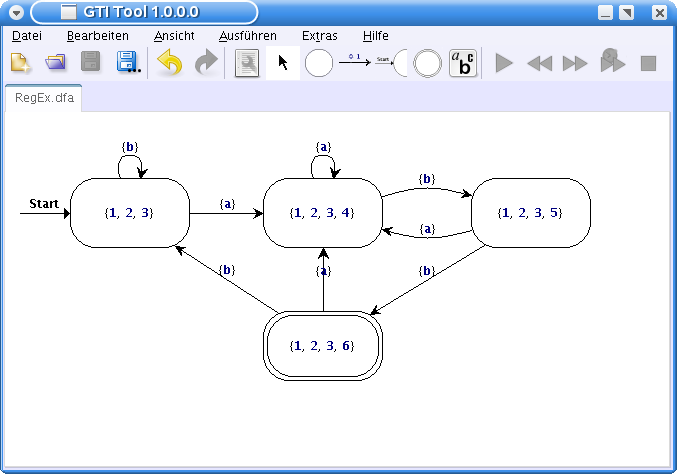
\includegraphics[width=12cm]{../images/regex_dfa.png}
\caption{Direkte Umwandlung in einen DEA}
\label{FigureRegExDFA}
\end{center}
\end{figure}
\vspace{10pt}


\section{\LaTeX-Export}\label{PerspectiveLaTeX}

Bei der Umsetzung des \gtitools war es uns in erster Linie wichtig, studentische
Benutzer zu unterstützen. Dazu zählt unter anderem das in Kapitel \ref{Print}
vorgestellte Drucken. Dadurch ist der Benutzer in der Lage, seine erstellten
Automaten oder Grammatiken auszudrucken, um so seine Unterlagen zu
vervollständigen. Eine weitere wichtige Funktion besteht in dem Bildexport.
Durch diesen Export ist der Benutzer in der Lage, die erstellten Automaten als
Bild zu exportieren, um sie zum Beispiel in eigene Prüfungsvorbereitungen
aufzunehmen.\vspace{10pt}

Als Perspektive für die Zukunft wäre es sinnvoll, auch Dozenten besser zu
unterstützen. Eine Möglichkeit wäre das Implementieren eines \LaTeX-Exports, so
dass der Lehrende nicht mehr den Umweg über den Bildexport gehen muss, sondern
den Automaten direkt in \LaTeX\ integrieren kann. Bei der Umsetzung ist auf die
Auswahl einer geeigneten \LaTeX-Bibliothek zu achten, so dass auch große
Automaten noch gut aussehen. Wichtig wäre auch, dass sich, wenn möglich, die
\LaTeX- und die am Bildschirm dargestellte Version wenig
unterscheiden.\vspace{10pt}


\section{Grammatik-Erweiterungen}\label{PerspectiveGrammar}

Bei Grammatiken gibt es noch diverse Möglichkeiten, welche bis jetzt noch nicht
umgesetzt sind. Als Beispiele, auf die wir in diesem Kapitel noch eingehen
möchten, haben wir uns Linksrekursion, Linksfaktorisierung und
Wort-Navigation auf einer Grammatik aufgegriffen.\vspace{10pt}


\subsection{Linksrekursion}\label{PerspectiveLeftrecursion}

Eine Grammatik wird als linksrekursiv bezeichnet, wenn sich aus einem beliebigen
Nichtterminalzeichen $\NonterminalSymbol{A}$ nach beliebig vielen Schritten etwas
von der Form $\NonterminalSymbol{A} \TerminalSymbol{$\alpha$}$ herleiten lässt.
Existiert eine Produktion $\NonterminalSymbol{A} \to \NonterminalSymbol{A}
\TerminalSymbol{$\alpha$}$ spricht man von direkter Linksrekursion. Wenn dazu
mehr als ein Ableitungsschritt nötig ist, spricht man von einer indirekten
Linksrekursion.\vspace{10pt}

%### removes texlipse warning
In \cite{Compilers} ist ein Algorithmus beschrieben, um Linksrekursion
bei einer Grammatik zu beseitigen, welcher sich ohne Probleme umsetzen lassen
sollte.\vspace{10pt}
%### removes texlipse warning

\noindent Gehen wir davon aus, die Produktionen für ein Nichtterminalzeichen
\NonterminalSymbol{A} sind von der Form\vspace{10pt}

\NonterminalSymbol{A} $\to$ \NonterminalSymbol{A}$\alpha_1|\ldots|$
\NonterminalSymbol{A}$\alpha_n | \beta_1 | \ldots | \beta_n$\vspace{10pt}

\noindent wobei $\beta_1\ bis\ \beta_n$ nicht mit \NonterminalSymbol{A}
beginnen.\vspace{10pt}

\noindent Um diese Rekursion zu beseitigen, führt man ein neues
Nichtterminalzeichen \NonterminalSymbol{A$'$} ein. Also ersetzt man die
bestehenden Produktion von
\NonterminalSymbol{A} durch diese Produktionen:\vspace{10pt}

\NonterminalSymbol{A} $\to \beta_1 | \ldots | \beta_n$

\NonterminalSymbol{A$'$} $\to \alpha_1$\NonterminalSymbol{A$'$}$|\ldots|$
$\alpha_n$\NonterminalSymbol{A$'$}$|\epsilon$\vspace{10pt}

%### removes texlipse warning
\noindent Damit können wir direkte Linksrekursion beseitigen. Und dies können wir
uns auch zunutze machen, um indirekte Linksrekursion zu entfernen. Folgender
Algorithmus zur Entfernung von Linksrekursion, aus dem Buch \cite{Compilers},
macht sich dies zu nutze:\vspace{10pt}
%### removes texlipse warning

\noindent
\verb| 1 for i = 1 to n do {|\\
\verb| 2   for j = 1 to i - 1 do {|\\
\verb| 3     ersetze jede Produktion der Form| $A_i \to A_j \gamma$ \verb| |\\ 
\verb| 4     durch die Produktion |$A_i \to \delta_1\gamma|\ldots|\delta_k\gamma$
\verb| 5 , wobei |$A_j \to \delta_1|\ldots|\delta_k$\\ 
\verb| 6     alle derzeitigen Produktionen für |$A_j$ \verb|sind|\\ 
\verb| 7   }|\\
\verb| 8   eleminiere die unmittelbare Linksrekursion für |$A_i$\\
\verb| 9   (mit dem vorhergehend beschriebenen Algorithmus)|\\
\verb|10 }|
\vspace{10pt}

Somit besteht die Möglichkeit sowohl direkte, wie auch indirekte Linksrekursion
zu beseitigen.\vspace{10pt}


\subsection{Linksfaktorisierung}\label{PerspectiveLeftfactorisation}

Bei einer Grammatik kann es zu Problemen kommen, wenn verschiedene Produktionen
gleiche Prefixe haben. Wie es zum Beispiel bei \vspace{10pt}

\noindent
\StartSymbol{S}$ \to$ \TerminalSymbol{if} \NonterminalSymbol{E} \TerminalSymbol{then}
\StartSymbol{S} \TerminalSymbol{else} \StartSymbol{S} $|$ 
\TerminalSymbol{if} \NonterminalSymbol{E} \TerminalSymbol{then} \StartSymbol{S}
\vspace{10pt}

\noindent
der Fall ist. Diese Probleme lassen sich durch den Algorithmus zur
Linksfaktorisierung lösen. Dieser Algorithmus sieht wie folgt aus.\vspace{10pt}

Zunächst einmal bestimmen wir eine Symbolfolge $\alpha$, welche dem längsten
gemeinsamen Prefix aller Produktionen für das selbe Nichtterminalzeichen
\NonterminalSymbol{A} entspricht. In unserem Beispiel wäre $\alpha$ 
"`\TerminalSymbol{if} \NonterminalSymbol{E} \TerminalSymbol{then}
\StartSymbol{S}"'. Alle Produktionen für \NonterminalSymbol{A} sind von der
Form\vspace{10pt}

\noindent
\NonterminalSymbol{A}$ \to \alpha \beta_1|\ldots|\alpha
\beta_n|\gamma_1|\ldots|\gamma_n$
\vspace{10pt}

\noindent
wobei $\gamma$ nicht mit $\alpha$ beginnt und es gilt $n \geq 2$ und $k \geq 0$.
\vspace{10pt}

Um den Algorithmus zur Linksfaktorisierung auf die Grammatik anzuwenden führt
man als erstes ein neus Nichtterminalzeichen \NonterminalSymbol{A$'$} ein. Als
nächstes ersetzt man die bestehenden Produktionen von \NonterminalSymbol{A}
durch die folgenden.\vspace{10pt}

\noindent
\NonterminalSymbol{A}$ \to \alpha $\NonterminalSymbol{A$'$}$|\gamma_1|\ldots|\gamma_n$\\
\NonterminalSymbol{A$'$}$ \to \beta_1|\ldots|\beta_n$
\vspace{10pt}

\noindent
Dieser Schritt muss wiederholt werden, bis für alle Produktionen mit dem
gleichen Nichtterminalzeichen auf der rechten Seite $\epsilon$ der einzige
gemeinsame Prefix ist.\vspace{10pt}

Dieser Algorithmus kann für eine Implementierung verwendet werden, indem für
jedes Nichtterminalzeichen überprüft, ob eine Linksfatorisierung nötig ist, und
diese dann wie oben beschrieben anwendet.


\subsection{Ableitungen für Grammatiken}\label{PerspectiveGrammarWordNavigation}

Die Wortnavigation für Automaten haben wir ja schon in Kapitel
\ref{WordNavigation} beschrieben. Etwas in der Richtung ließe sich
auch für Grammatik realisieren. Allerdings naviert man nicht mehr
durch ein Wort, sondern man sucht die richtig Ableitung von dem
Startsymbol aus.\vspace{10pt}

Dazu könnte die Top-Down Methode des rekursiven Abstiegs verwendet werden. Dieser
Algorithmus startet mit dem Startsymbol der Grammatik auf dem Keller. Wenn
mehrere Produktionen für das Startsymbol in der Grammatik existieren, muss der
Benutzer jetzt auswählen, welches die richtige Produktion ist. Dann wird das
Startsymbol durch die rechte Seite dieser Produktion ersetzt. Jetzt nimmt man
sich jedes Symbol einzeln vor, wobei man von links startet. Handelt es sich um
ein Nichtterminalzeichen, würde dieses wieder durch die rechte Seite der
richtigen nächsten Produktion ersetzt. Handelt es sich um ein Terminalzeichen,
wird dieses mit dem nächsten Zeichen im Eingabewort verglichen. Wenn diese
übereinstimmen wird ein Pointer innerhalb des Eingabewortes ein Symbol
weitergeschoben, und man betrachtet das nächste Symbol. Wenn die beiden Symbole
nicht übereinstimmen, muss eine Fehlermeldung ausgegeben werden, dass dieses Wort
mit den bis jetzt verwendeten Produktionen nich hergeleitet werden kann. Wenn man
das letzte Symbol auf dem Keller behandelt hat, sollte auf dem Keller das
Eingabewort stehen. Somit kann man das Wort mit den Produktionen herleiten, die
man während dieses Durchlaufs verwendet hat. Als Hilfestellung für den Benutzer
sollten diese noch in einer Liste, oder etwas ähnlichem in der Reihenfolge der
Verwendung aufgelistet werden.\vspace{10pt}

\section{Erkannte Wörter ausgeben}\label{PerspectiveDetectedWords}

Eine weitere sinnvolle und für die Zukunft angedachte Erweiterung ist die Ausgabe
von erkannten Wörtern. Nachdem ein Automat, eine Grammatik oder ein regulärer
Ausdruck eingebenen und validiert wurde, soll der Benutzer in der Lage sein, eine
Ansicht zu öffnen, in der er Wörter ausgegeben bekommt, die zum Beispiel von dem
erstellten Automaten erkannt werden.\vspace{10pt}

Bei der Umsetzung ist darauf zu achten, dass die Bestimmung dieser Wörter
möglichst mit geringer Laufzeit implementiert wird, so dass der Benutzer nicht
allzu lange auf ein Ergebnis warten muss. Die Bestimmung sollte somit nicht
einfach per Brute-Force-Methode umgesetzt werden, sondern in irgendeiner Form
abhängig von dem gewendeten Typ sein, wie zum Beispiel einer Grammatik. Somit
sollten gewisse Wörter direkt ausgeschlossen werden, die bei der
Brute-Force-Methode ansonsten mit getestet werden würden.\vspace{10pt}


\section{Eingabe von mehreren Wörtern}\label{PerspectiveMultiplyWordInput}

In der aktuellen Version des \gtitools kann man für Automaten nur ein Wort
eingeben. In Zukunft soll diese Eingabe aber auch für Grammatiken und dann auch
für reguläre Ausdrücke möglich sein. In der aktuellen Umsetzung kann der Benutzer
aber nur ein Wort eingeben und dieses dann auf Akzeptanz prüfen. Für zukünftige
Versionen wäre es somit wünschenswert, mehr als ein Wort eingeben zu können,
welches dann direkt während der Eingabe überprüft wird, so dass der Benutzer
nicht erst die Navigation starten muss. Diese Ansicht soll dem Benutzer helfen,
zu erkennen, welche Sprache ein erstellter Automat oder eine Grammatik
erkennt.\vspace{10pt}

Eine mögliche Umsetzung wäre, dass Wörter in einer editierbaren Tabelle
eingegeben werden können. Dazu wäre in jeder Zeile ein Parser nötig, der die
Wörter erkennt. Wird eine gültige Eingabe gemacht, kann der Automat dazu
benutzt werden, dieses Wort auf Akzeptanz zu prüfen.\vspace{10pt}


\section{Benutzerinteraktion erhöhen}\label{PerspectiveInteraction}

Bei der Umsetzung des \gtitools war es uns sehr wichtig, dass der Benutzer bei
der Verwendung des Programms möglichst viel lernt. Im Kapitel \ref{Concepts}
wurden einige Konzepte angesprochen, die uns bei der Umsetzung sinnvoll
erschienen. Aufgrund des vermutlich sehr großen Aufwandes konnten wir den Bereich
Benutzerinteraktion nicht weiter ausbauen. In diesem Abschnitt werden mögliche
Anpassungen angesprochen, die für zukünftige \gtitool Versionen geplant sind. Bei
diesen Anpassungen handelt es sich zum größten Teil um Erweiterungen der schon
implementierten Umsetzungen. Alle in der Zukunft implementierten Erweiterungen
sollten dann direkt mit einer entsprechend hohen Benutzerinteraktion umgesetzt
werden, so dass das nachträgliche Erweitern entfallen würde.\vspace{10pt}


\subsection{Word-Navigation}\label{PerspectiveWordNavigation}
Eine wichtige Erweiterung betrifft die Wort-Navigation. Bei dieser Navigation
gibt es bereits eine Benutzerinteraktion, welche in Abschnitt
\ref{InteractionPDA} beschrieben wird. In Zukunft kann die Benutzerinteraktion,
die in Abschnitt \ref{WordNavigation} beschrieben wird, erweitert werden. Eine
mögliche Umsetzung wäre, den Benutzer vor einem Navigationsschritt dazu
aufzufordern, die Übergänge zu markieren, die als nächstes verwendet werden.
Dabei müsste der Benutzer anhand des nächsten Symbols im Eingabewort entscheiden,
welche Übergänge dies betrifft. Kommen ein oder mehrere $\epsilon$-Übergänge vor,
müssen diese Übergänge zuerst ausgewählt werden. Durch diese Erweiterung würde
der Benutzer noch besser erkennen können, wie der Algorithmus arbeitet. Um den
ungeübten Benutzer nicht zu überfordern und somit vielleicht zur Aufgabe zu
zwingen, muss dieser zusätzliche Auswahlschritt überspringbar sein. Es muss also
eine Art "`Raten-Funktion"' geben, die dem Benutzer die Auswahl
abnimmt.\vspace{10pt}


\subsection{Konvertierung}\label{PerspectiveConvertTo}
Im Abschnitt \ref{ConverToMachine} wird das Umwandeln eines Automaten in einen
anderen Automaten beschrieben, also zum Beispiel die Umwandlung von einem
$\epsilon$-NDEA in einen DEA. Der dort implementierte Algorithmus verwendet
verschiedene Phasen. Eine dieser Phasen ist das Bilden des
$\epsilon$-Abschlusses. In diesem Schritt wäre es möglich, den Benutzer alle
Zustände markieren zu lassen, die von dem aktiven Zustand nur durch
$\epsilon$-Übergänge erreichbar sind.\vspace{10pt}

Eine weitere Möglichkeit wäre, den Benutzer dazu aufzufordern, die Zustände zu
aktivieren, die nach einem Übergang mit einem bestimmten Symbol aktiviert sein
werden. Aber auch bei allen anderen Phasen sollte geprüft werden, ob es sinnvoll
wäre, den Benutzer zu einer Interaktion aufzufordern. Es wäre aber nicht nur
möglich, Zustände und Übergänge in dem ursprünglichen Graphen zu markieren,
ebenso wäre es in dem entstehenden Graphen möglich, anzugeben, welche Zustände und
Übergänge in dem nächsten Schritt angelegt werden.\vspace{10pt}


\subsection{Erreichbare Zustände}\label{PerspectiveReachableStates}
Wie im Abschnitt \ref{ReachableStates} vorgestellt, implementiert der
Algorithmus zur Bestimmung der erreichbaren Zustände eine Breitensuche. Bei
dieser Breitensuche könnte der Benutzer dazu aufgefordert werden, die
erreichbaren Zustände zu markieren. Diese Markierung könnte dann überprüft
werden und der Benutzer würde über die Richtigkeit seiner Eingabe informiert.
Auch bei dieser Benutzerinteraktion wäre eine Funktion wichtig, die die
richtige Auswahl trifft.\vspace{10pt}


\subsection{Minimierung}\label{PerspectiveMinimize}
Das Minimieren von Automaten bietet sehr großen Spielraum zum Einbau von
Benutzerinteraktion. Der in Kapitel \ref{Minimize} vorgestellte Algorithmus
basiert darauf, Zustände in Äquivalenz\-klassen zu unterteilen. Es wäre somit
möglich, diese Unterteilung dem Benutzer zu überlassen. Er müsste also
auswählen, warum eine Gruppe in zwei Gruppen zerfällt. Um dies zu erreichen,
müsste der Benutzer Übergänge mit dem gleichen Symbol finden, die in
unterschiedlichen Gruppen enden.\vspace{10pt}

Im ersten Schritt des Minimierens werden die nicht erreichbaren Zustände
entfernt, auch diesen Schritt kann der Benutzer selbst durchführen, in dem er die
entsprechenden Zustände auswählt.\vspace{10pt}


\section{Auto-Layout}\label{PerspectiveAutoLayout}

%###
Wie im Kapitel \ref{AutoLayout} schon erwähnt ist kann der implementierte
Autolayout-Algorithmus noch optimiert werden. Ein Algorithmus welcher
wahrscheinlich bessere Ergebnisse liefert ist der
Simulated-Annealing-Algorithmus (Simulierte Abkühlung), welcher auch in \cite{Layout} beschrieben
wird.\vspace{10pt}
%###

Bei diesem Algorithmus versucht man sich das Verfahren des Abkühlungsprozesses zu
Nutze zu machen, welches in der Natur beobachtet werden kann. Wenn man diesen
Prozess Beispielsweise bei metallischen Schmelzen beobachtet, kann man
feststellen, dass die Metallatome sich zu Beginn des Abkühlunsprozesses noch
annähernd chaotisch durch die Gitterpositionen bewegen. Mit abnehmender
Temperatur nehmen die Atome allerdings immer mehr geordnete Positionen ein, so
dass später nur noch eine Optimierung in der lokalen Nachbarschaft der Atome
möglich ist. Durch dieses Verfahren wird in der Natur immer eine
optimal Lösung erreicht, weshalb man versucht dieses auf ein
Partitionierungsproblem zu übertragen.\vspace{10pt}

Diesen, in der Natur beobachteten Algorithmus, versucht man jetzt nachzubilden,
und mit diesem Verahren Partitionierungsprobleme, beziehungsweise
Layoutprobleme, zu lösen. Dabei gibt man den Elementen zu Beginn einen hohen
Freiheitsgrad, wie es ja auch bei dem Abkühlungsprozess der Fall ist. Dadurch
nimmt man auch Verschlechterungen in Kauf. Dieser Freiheitsgrad nimmt jedoch
immer weiter ab, so dass die Akzeptanz von Verschlechterungen immer weiter
sinkt.\vspace{10pt}

Bei dem Algorithmus werden die Elemente zu Beginn in einer zufällige
Anfangspositionierung gebracht. Jetzt wird über eine Kostenfunktion die
aktuellen Kosten bei dieser Konfiguration berechnet. Als nächstes wählt man
willkürlich zwei Elemente aus und berechnet erneut die Kosten für den Fall,
dass man diese beiden Elemente tauschen würde. Wenn sich die Kosten verbessern
wird der Tausch auf jeden Fall durchgeführt. Wenn die Kosten gleich bleiben,
oder sich sogar verschlechtern würden tauscht man mit einer bestimmten
Wahrscheinlichkeit. Die Maßgebenden Faktoren zur Berechnung der
Wahrscheinlichkeit sind die aktuelle Temperatur und der Grad der
Veschlechterung.\vspace{10pt}

\noindent
Der Pseudocode für diesen Algorithmus sieht wie folgt aus:\vspace{10pt}

\noindent
\verb| 1 begin|\\
\verb| 2   T = T|$_0$\verb|, i = 0|\\
\verb| 3   cur_part = init_part|\\
\verb| 4   cur_cost=COST( cur_part )|\\
\verb| 5   repeat|\\
\verb| 6     repeat|\\
\verb| 7       i = i + 1|\\
\verb| 8       a|$_i$\verb| = SELECT( A ), b|$_i$\verb| = SELECT( B )|\\
\verb| 9       trial_part = EXCHANGE( a|$_i$\verb|,b|$_i$\verb|, cur_part )|\\
\verb|10       trial_cost = COST( trial_part )|\\
\verb|11       |$\Delta$\verb|cost = trial_cost - cur_cost|\\
\verb|12       if ( |$\Delta$\verb|cost < 0 ) then|\\
\verb|13         cur_cost = trial_cost|\\
\verb|14         cur_part = MOVE ( a|$_i$\verb|, b|$_i$\verb| )|\\
\verb|15       else|\\
\verb|16         r = RANDOM ( 0, 1 )|\\
\verb|17         if ( r < e|$^{-\frac{\Delta cost}{T}}$\verb| ) then|\\
\verb|18           cur_cost = trial_cost|\\
\verb|19           cur_part = MOVE ( a|$_i$\verb|, b|$_i$\verb| )|\\
\verb|20     until (Abbruchskriterium, z.B. Gleichgewicht bei T, erreicht)|\\
\verb|21    T = |$\alpha$\verb| * T|\\
\verb|22   until ( T < T|$_{min}$\verb| )|\\
\verb|23 end|\\ 
\vspace{10pt}

Die Kostenfunktion ist bei der Implementierung des Algorithmus ein wichtiger
Punkt aus. In unserem speziellen Fall müsste man berücksichtigen, dass zwei
Zustände, zwischen denen ein Übergang existiert, nicht zu weit auseinanderliegen
sollten. Wenn zwei Zustände nicht direkt nebeneinander liegen können, sollte sehr
großer Wert darauf gelegt werden, dass der Übergang nicht durch einen anderen
Zustand geht, so dass die Beschriftung des Übergangs oder des anderen Zustandes
eventuell nicht mehr zu erkennen ist. Weiterhin sollten die Überschneidungen der
Übergänge untereinander möglichst gering sein.
\vspace{10pt}
